\subsection{Printed Circuit Board Design} \label{sec:pcb-design}
\noindent FORWARD requires the use of two printed circuit board designs: PCB 1) includes sensors, MCU, and Bluetooth support, and PCB 2)  is velocity and haptic control.

\noindent On PCB 1, it is advantageous to use the 5V configuration for ESP32 UART bridge. In development, we used a development board to program the MCU but in practice must implement a UART bridge on the PCB to communicate with the MCU for flashing the memory and sending serial data out. On PCB 1, we have surface mount components and sockets for all the sensors, as well as the communication connections to the motor shields on PCB 2.  Note that, almost all of the GPIO pins on the microcontroller are filled!\\

\noindent Also on PCB 1, for voltage regulation, it is expedient to, instead of using Texas Instruments Webench to design regulator circuits, use a 2/3 voltage divider for the ultrasonic ECHO pins. This is necessary because the ESP32 operates on 3.3V while the ultrasonic sensors use 5V, even though they are 3.3V compatible. As observed in system testing, only supplying 3.3 volts leads to signal bouncing. This can be easily implemented by a 1k$\Omega$ and 2k$\Omega$ resistor in series. One other consideration are the PCB traces. We intend to use 20mil (0.5mm) isolations and traces. Under consideration is the inclusion of RF circuitry to allow the data network to still operate.\\

\begin{figure}[H]
	\centering
	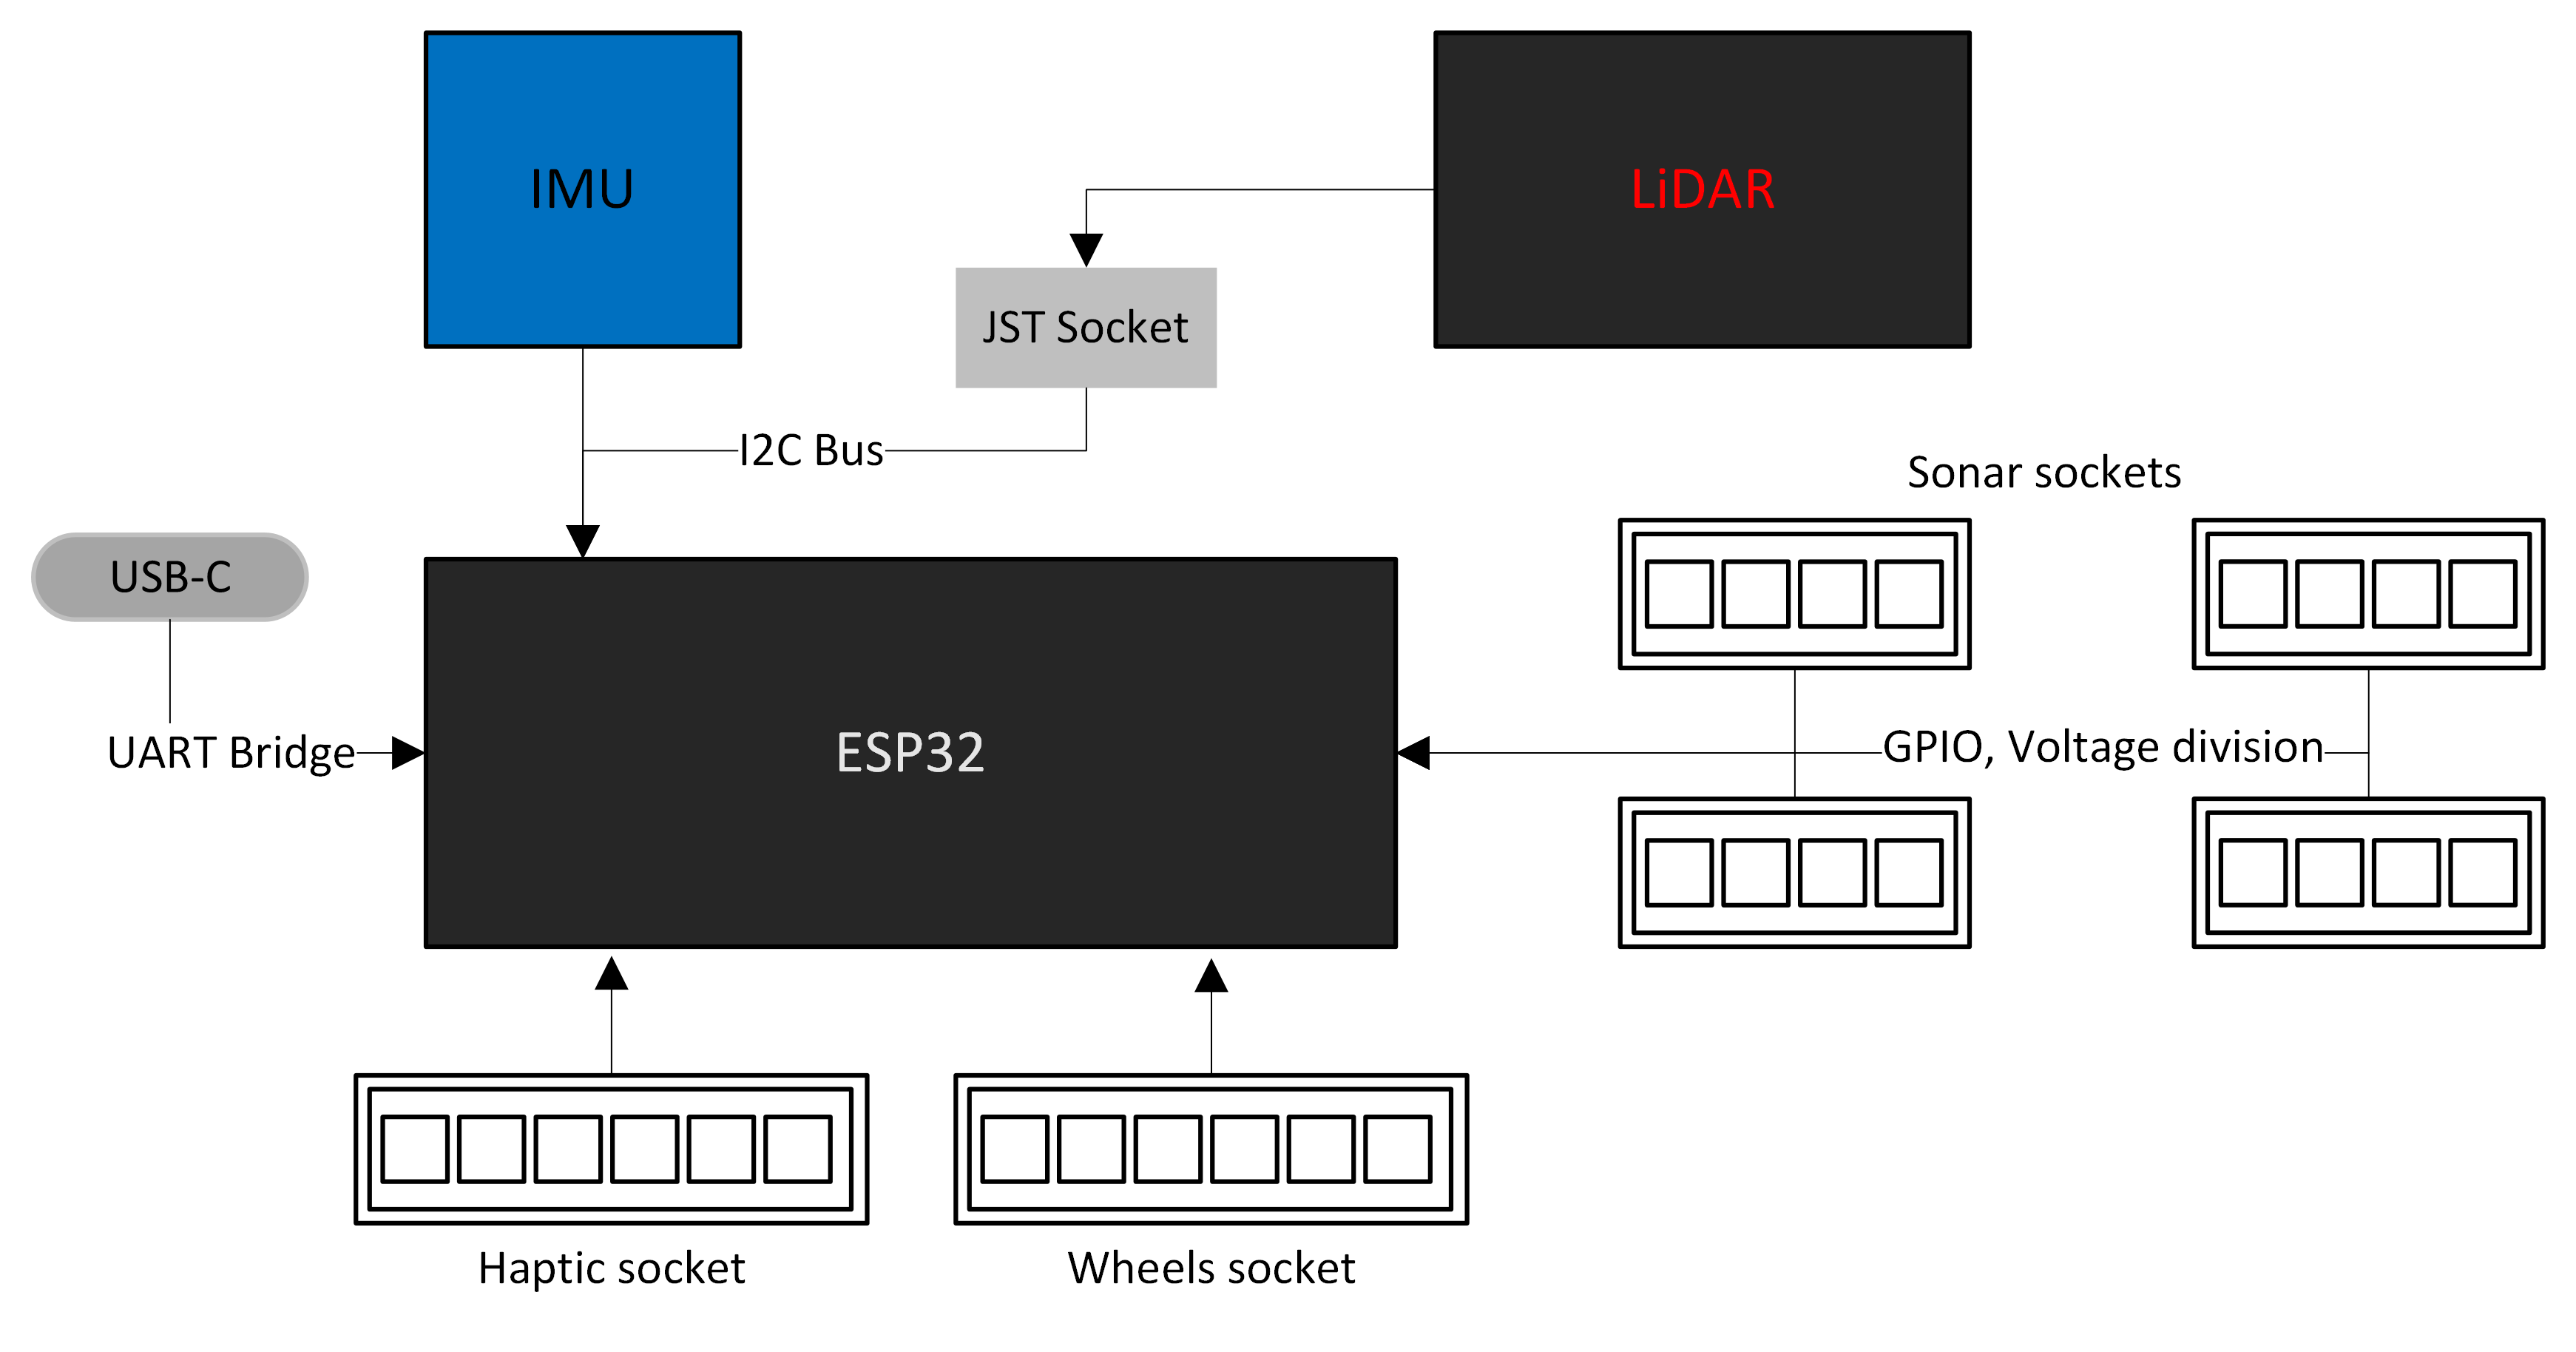
\includegraphics[width=\textwidth]{./Images/PCB1-Block-Diagram.png}
	\caption{\label{fig:pcb}PCB 1 Block Diagram}
\end{figure}

\begin{figure}[H]
	\centering
	\includegraphics[width=\textwidth]{./Images/PCB1-sch.png}
	\caption{\label{fig:pcb-sch}PCB KiCAD Schematic}
\end{figure}


\begin{figure}[H]
	\centering
	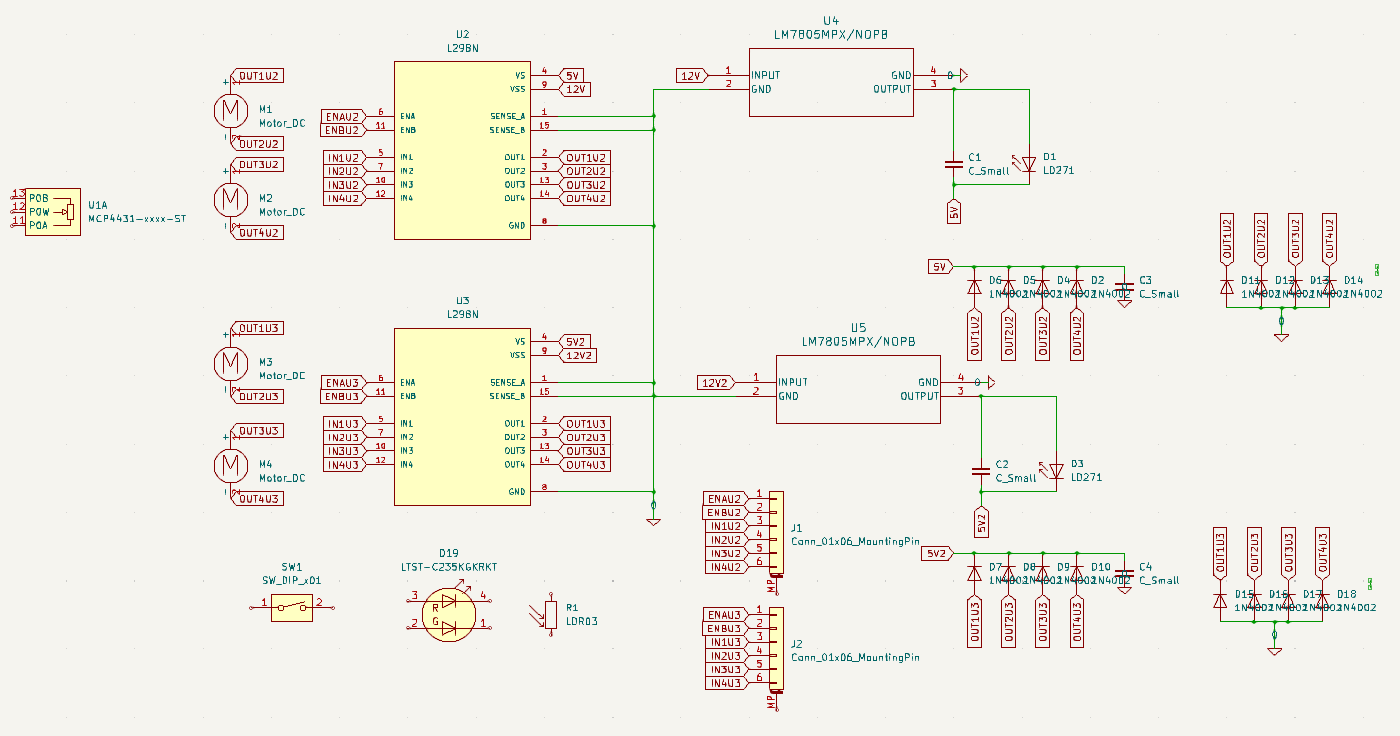
\includegraphics[width=\textwidth]{./Images/pcb-avoidance-headers.png}
	\caption{\label{fig:pcb-motor}PCB KiCAD Schematic for Avoidance Subsytem}
\end{figure}

\noindent Motor controllers are more sensitive components and should be implemented on an independent PCB. These are considered as optically isolated motor drivers in order to minimize back EMI/F. In this case, one would bias an LED to turn the controller on. This is why PCB 2 is separated, and it includes a potentiometer, headlights, and other components necessary for obstacle avoidance\\

